%% MSR 2027 -- Data and Tool Showcase Track
%% 4 pages + 1 page references. IEEE conference format.
\documentclass[conference]{IEEEtran}
\IEEEoverridecommandlockouts
\usepackage{cite}
\usepackage{amsmath,amssymb,amsfonts}
\usepackage{graphicx}
\usepackage{booktabs}
\usepackage{url}
\usepackage[hidelinks]{hyperref}
\usepackage{listings}
\lstset{basicstyle=\ttfamily\scriptsize,breaklines=true,frame=single,columns=fullflexible}

\begin{document}

\title{codehound: A Zero-Dependency AST Analyzer for\\Async-Safety and Resource Defects in Python AI/ML Frameworks}

\author{
\IEEEauthorblockN{Abhinav Tarigoppula}
\IEEEauthorblockA{\textit{Dept. of Computer Science \& Engineering}\\
\textit{GITAM University}\\
Visakhapatnam, India\\
abhinaaavvv07187@gmail.com}
}

\maketitle

\begin{abstract}
The infrastructure of contemporary machine learning---model-serving engines, agent frameworks, and LLM tool integrations---is written predominantly in Python and increasingly built on \texttt{asyncio}. Asynchronous Python concentrates a family of defects that raise no exception, pass unit tests, and surface only under production load or particular garbage-collection timing. We present \textbf{codehound}, a zero-dependency static analyzer (${\approx}750$ LOC, standard-library \texttt{ast} only) that detects six such defect classes, together with a dataset of its findings across 28 widely-used Python AI/ML frameworks (1.3M combined GitHub stars, 6.4M lines of Python), in which it identifies 1{,}377 defect instances in 24 of the 28 projects. The artifact is distinguished from typical tool releases by its external validation: fixes derived from its detections were reviewed and \emph{merged upstream by maintainers} of eight pull requests across six organizations, spanning three rule classes. We release the analyzer, the full scan dataset, and the table of accepted fixes under MIT licence with a persistent DOI, so that both the tool and the evidence for its precision can be reused and independently checked.
\end{abstract}

\begin{IEEEkeywords}
static analysis, abstract syntax trees, asyncio, concurrency defects, resource leaks, mining software repositories, machine-learning infrastructure
\end{IEEEkeywords}

\section{Introduction}
\texttt{asyncio} is cooperative, single-threaded concurrency: one event loop interleaves many tasks and switches only at \texttt{await} points. Between awaits, whatever runs monopolizes the loop. That single property underlies a class of defects which are unusually hard to observe dynamically. A synchronous \texttt{time.sleep} inside an \texttt{async def} freezes every in-flight request; a task created with a bare \texttt{asyncio.create\_task(...)} whose handle is discarded may be garbage-collected before it completes, so the work silently never happens. Neither raises an exception, and neither fails a unit test.

These patterns are well understood in principle, yet we found them in production paths of some of the most heavily used AI frameworks on GitHub. That they persist there is consistent with two established observations: that real-world concurrency defects concentrate in a small number of recurring patterns rather than exotic ones~\cite{lu2008}, and that machine-learning systems accumulate maintenance burden in the ordinary software surrounding the model rather than in the model itself~\cite{sculley2015}. Empirical work on deep-learning frameworks has likewise found defect classes that produce no crash and no error message, and so survive testing~\cite{silentbugs,dlbugs}; the defects we target share that property.

This artifact paper contributes:

\begin{enumerate}
  \item \textbf{codehound}, an open-source, zero-dependency AST analyzer detecting six concurrency- and resource-management defect classes (Section~\ref{sec:tool}).
  \item \textbf{A reusable dataset} of per-repository, per-rule findings across 28 popular Python AI/ML frameworks, with pinned commits for reproducibility (Section~\ref{sec:dataset}).
  \item \textbf{A ground-truth table of maintainer-accepted fixes}: eight upstream pull requests merged across six organizations, each linked to the rule that produced it (Section~\ref{sec:validation}).
\end{enumerate}

The third contribution is what we believe makes the artifact reusable beyond our own study. Static-analysis tools are routinely evaluated on synthetic benchmarks or by author-adjudicated sampling. Here, precision is evidenced by the decisions of maintainers who had no stake in the tool and who accepted the resulting patches into shipping software.

\section{Detected Defect Classes}
codehound implements six checks, each distilled from a defect the author first found and fixed in a widely-used framework.

\begin{itemize}
  \item \textbf{CH001 --- blocking call in async context.} A synchronous, latency-bearing call (e.g.\ \texttt{time.sleep}, \texttt{requests.get}) evaluated inside an \texttt{async def} without \texttt{await}.
  \item \textbf{CH002 --- mutable default argument.} A parameter defaulting to a mutable literal, sharing one object across all invocations (cf.\ \texttt{flake8-bugbear} B006).
  \item \textbf{CH003 --- deprecated \texttt{datetime.utcnow()}.} Returns a na\"ive datetime; deprecated since Python 3.12.
  \item \textbf{CH004 --- deprecated \texttt{asyncio.get\_event\_loop()}.} Deprecated outside a running loop.
  \item \textbf{CH005 --- unclosed file handle.} An \texttt{open()} whose result is neither used as a context manager nor explicitly closed.
  \item \textbf{CH006 --- fire-and-forget task.} A bare expression-statement call to \texttt{create\_task}/\texttt{ensure\_future} whose result is discarded, permitting mid-run garbage collection (cf.\ Ruff RUF006).
\end{itemize}

\section{Tool Design}
\label{sec:tool}
codehound parses each file with the standard-library \texttt{ast} module and precomputes a child$\rightarrow$parent map, which Python's \texttt{ast} does not record. That map supports the upward scope queries the checks depend on: \emph{which function encloses this node?}, \emph{is this call the operand of an \texttt{await}?}, and \emph{is this statement inside a \texttt{with} block?} Each rule is an independent \texttt{Check} subclass emitting \texttt{Finding(path, line, col, code, message)} records, so rules can be enabled individually and new ones added without touching the traversal.

Two design decisions target precision rather than recall, and both were motivated by false positives observed during upstream submission. CH001 ignores awaited calls, so \texttt{await client.get(...)} is not flagged merely because the receiver resembles a synchronous library. CH006 flags only bare expression statements, so a task assigned to a variable, awaited, returned, or handed to a \texttt{TaskGroup} is not reported. Deliberately, codehound has no third-party dependencies: it runs anywhere a Python interpreter runs, which matters for scanning a large corpus of projects with mutually incompatible dependency trees.

\subsection{Relation to existing linters}
Mature linters already cover parts of this space, and we do not claim otherwise: \texttt{flake8-bugbear}~\cite{bugbear} B006 detects mutable defaults, and Ruff~\cite{ruff} implements both that rule and RUF006 for discarded task handles, alongside an \texttt{ASYNC} family targeting blocking calls. Where those tools are engineered as general-purpose linters configured per project, codehound is engineered as a \emph{corpus instrument}. Three properties follow from that goal. It has no third-party dependencies and no configuration file, so it can be pointed at hundreds of unrelated repositories without resolving each project's toolchain. It emits a flat, machine-readable record per finding, which is what makes a cross-repository dataset cheap to assemble. And its rule set is deliberately small and fixed, so counts are comparable across repositories without normalising for divergent per-project lint configuration---a project that disables B006 in its own \texttt{pyproject.toml} still contributes CH002 counts here.

The practical consequence is that our contribution is not a better mutable-default detector. It is a reproducible pipeline from ``popular Python AI/ML projects'' to ``a comparable per-rule defect table,'' plus the evidence in Section~\ref{sec:validation} that the findings it surfaces are ones maintainers act on.

\begin{lstlisting}[caption={Scanning a repository for two rule classes.}]
$ PYTHONPATH=codehound/src python3 -m codehound.cli \
      scan /path/to/repo --select CH001,CH006

repo/serving/api.py:214:9 CH001 blocking call
    'time.sleep' inside async function 'export_model'
repo/engine/abort.py:88:5 CH006 result of
    'asyncio.create_task' is discarded
\end{lstlisting}

By default the analyzer skips test, example, and documentation directories, focusing on production code paths where these defects have consequence.

\section{The Dataset}
\label{sec:dataset}
We shallow-cloned 28 popular open-source Python AI/ML projects---spanning model serving, agent frameworks, LLM tooling, RAG, and training---pinned each to a specific commit, and ran all six checks. The corpus comprises 1{,}299{,}231 combined GitHub stars and 6{,}386{,}365 lines of analyzed Python.

\texttt{corpus\_scan\_results.csv} records one row per repository: the pinned commit, star count, Python LOC analyzed, per-rule counts, and total. Pinning commits means every number in Table~\ref{tab:dist} is recomputable from the raw file.

\begin{table}[t]
\caption{Defect instances by rule across the 28-project corpus.}
\label{tab:dist}
\centering
\begin{tabular}{llrr}
\toprule
\textbf{Rule} & \textbf{Defect class} & \textbf{Count} & \textbf{Share} \\
\midrule
CH002 & mutable default argument   & 742 & 53.9\% \\
CH004 & deprecated \texttt{get\_event\_loop} & 286 & 20.8\% \\
CH006 & fire-and-forget task        & 262 & 19.0\% \\
CH003 & deprecated \texttt{utcnow}  &  55 &  4.0\% \\
CH001 & blocking call in async      &  22 &  1.6\% \\
CH005 & unclosed file handle        &  10 &  0.7\% \\
\midrule
\multicolumn{2}{l}{\textbf{Total}}  & \textbf{1{,}377} & \\
\bottomrule
\end{tabular}
\end{table}

\begin{figure}[t]
\centering
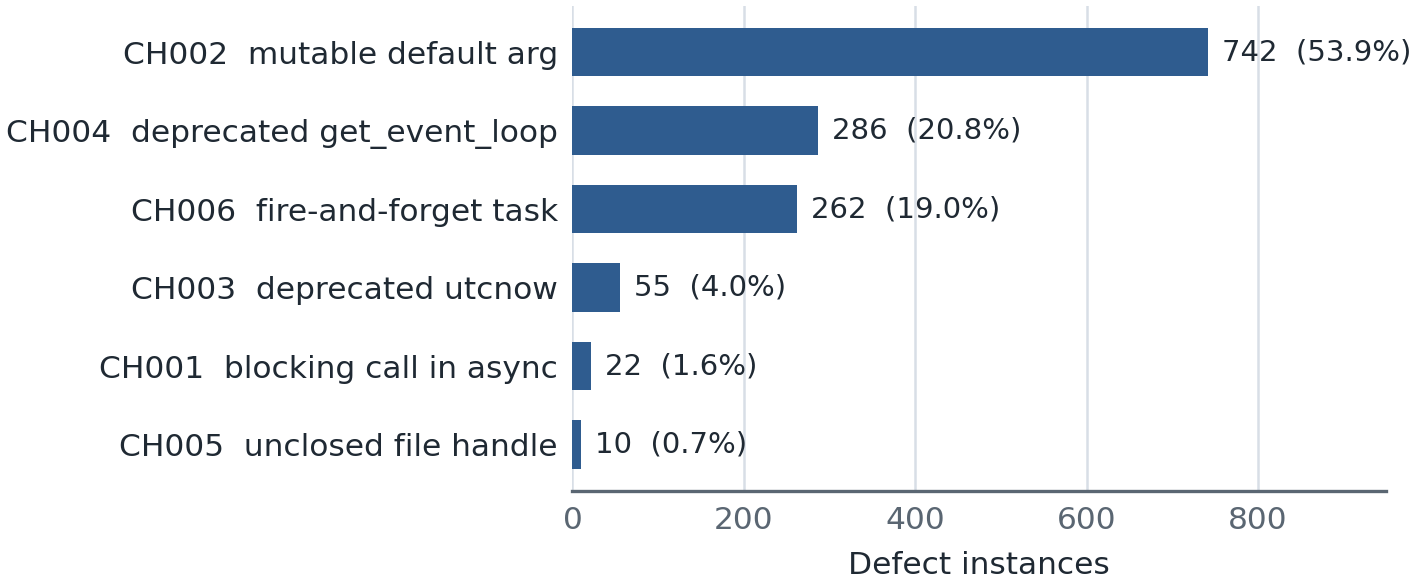
\includegraphics[width=\columnwidth]{figures/fig1_defects_by_class.png}
\caption{Defect instances by rule across the 28-project corpus.}
\label{fig:byclass}
\end{figure}

\begin{figure}[t]
\centering
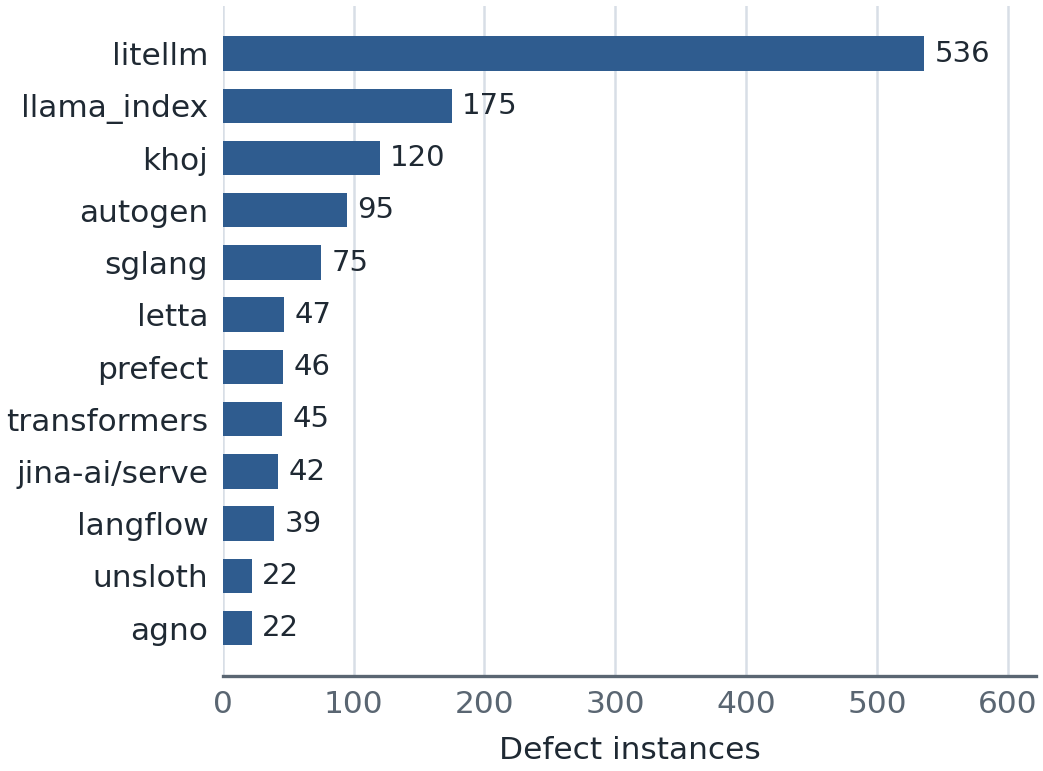
\includegraphics[width=\columnwidth]{figures/fig2_top_frameworks.png}
\caption{The twelve most affected projects, by total defect instances.}
\label{fig:topframeworks}
\end{figure}

We identified 1{,}377 defect instances in 24 of the 28 projects. The distribution is heavily skewed (Fig.~\ref{fig:byclass}): CH002 alone accounts for over half of all findings, while CH001---the class with the most direct production impact, since one blocking call stalls every concurrent request---is comparatively rare at 22 instances. That asymmetry is itself a useful signal for practitioners: the most common defect is not the most costly one.

Findings are also concentrated by project (Fig.~\ref{fig:topframeworks}). A single project accounts for 536 of the 1{,}377 instances, and the four most affected account for roughly two thirds. Concentration of this kind is expected---it tracks codebase size and how heavily a project leans on \texttt{asyncio}---but it means aggregate counts should not be read as a per-project quality ranking. Both figures are regenerated directly from the released CSV by \texttt{make\_figures.py}.

One repository was excluded from the analysis set and the reasoning recorded in \texttt{EXCLUSIONS.md}. At its pinned commit it tracked no Python source, delegating all implementation to four submodules; it had been recorded with zero findings, which is a non-observation rather than a clean result, and retaining it would have inflated the denominator of every prevalence figure.

\section{Prior Applications and Validation}
\label{sec:validation}
Static counts cannot establish that a flagged pattern is a defect the community considers worth fixing. We therefore submitted a sample of detections as upstream pull requests and treated maintainer acceptance as ground truth.

\begin{table}[t]
\caption{Maintainer-accepted fixes derived from codehound detections.}
\label{tab:merged}
\centering
\begin{tabular}{llr}
\toprule
\textbf{Rule} & \textbf{Project} & \textbf{PR} \\
\midrule
CH001 & unslothai/unsloth              & \#6135 \\
CH001 & agno-agi/agno                  & \#8158 \\
CH001 & agno-agi/agno                  & \#8186 \\
CH001 & xorbitsai/inference            & \#5055 \\
CH001 & weaviate/weaviate-python-client& \#2104 \\
CH002 & mem0ai/mem0                    & \#5302 \\
CH002 & pydantic/pydantic-ai           & \#6189 \\
CH005 & agno-agi/agno                  & \#8161 \\
\bottomrule
\end{tabular}
\end{table}

Eight pull requests were merged by maintainers across six organizations, spanning three of the six rule classes (Table~\ref{tab:merged}). \texttt{merged\_fixes.csv} records each with its rule, repository, star count, public pull-request URL, and merge date, so every row can be verified independently.

We make a deliberately narrow claim. These eight are the fixes attributable to a codehound detection; other contributions by the author to the same ecosystem---documentation, features, and issue-driven logic fixes---are excluded, because they are not evidence about this tool. Acceptance also establishes that a finding was actionable in a maintainer's judgement; it is a lower bound on precision, not a measurement of recall, and rules with no accepted fix are unevidenced rather than disproven.

\section{Limitations}
The analyzer is purely syntactic. It performs no type inference or interprocedural analysis, so CH001 relies on a curated list of known-blocking call targets and will miss a blocking call reached indirectly through a helper. CH005 cannot track a handle stored on an object and closed elsewhere. The corpus is a convenience sample of popular projects and is not a random sample of Python AI/ML software, so the prevalence figures describe this corpus rather than the ecosystem. Validation covers three of six rules; CH003, CH004, and CH006 have no maintainer-accepted fix in this dataset. In particular, CH004 detections are frequently intentional---\texttt{get\_event\_loop()} inside an already-running loop is well-defined---and we regard that rule as advisory.

\section{Availability}
codehound and the complete dataset are released under the MIT licence and archived with a persistent DOI:

\begin{itemize}
  \item \textbf{DOI:} \url{https://doi.org/10.5281/zenodo.21851079}
  \item \textbf{Repository:} \url{https://github.com/kratos0718/codehound}
\end{itemize}

The archive contains the analyzer source and test suite, CI configuration for Python 3.9--3.12, \texttt{corpus\_scan\_results.csv}, \texttt{merged\_fixes.csv}, \texttt{EXCLUSIONS.md}, and the figures. The DOI above is a concept DOI resolving to the latest version; individual releases carry their own version DOIs.

\section*{Acknowledgment}
The author thanks the maintainers of the projects listed in Table~\ref{tab:merged} for reviewing the submitted patches.

\begin{thebibliography}{9}
\bibitem{lu2008} S. Lu, S. Park, E. Seo, and Y. Zhou, ``Learning from mistakes: A comprehensive study on real world concurrency bug characteristics,'' in \emph{Proc. 13th Int. Conf. Architectural Support for Programming Languages and Operating Systems (ASPLOS)}, 2008.
\bibitem{sculley2015} D. Sculley, G. Holt, D. Golovin, E. Davydov, T. Phillips, D. Ebner, V. Chaudhary, M. Young, J.-F. Crespo, and D. Dennison, ``Hidden technical debt in machine learning systems,'' in \emph{Advances in Neural Information Processing Systems (NIPS)}, 2015.
\bibitem{silentbugs} F. Tambon, A. Nikanjam, L. An, F. Khomh, and G. Antoniol, ``Silent bugs in deep learning frameworks: An empirical study of Keras and TensorFlow,'' \emph{Empirical Software Engineering}, 2024. arXiv:2112.13314.
\bibitem{dlbugs} J. Chen \emph{et al.}, ``A comprehensive empirical study on bug characteristics of deep learning frameworks,'' \emph{Information and Software Technology}, vol.~151, 2022.
\bibitem{asyncio} Python Software Foundation, ``asyncio --- Asynchronous I/O,'' Python Standard Library Documentation. \url{https://docs.python.org/3/library/asyncio.html}
\bibitem{ruff} Astral, ``Ruff: An extremely fast Python linter and code formatter,'' \url{https://github.com/astral-sh/ruff}
\bibitem{bugbear} PyCQA, ``flake8-bugbear,'' \url{https://github.com/PyCQA/flake8-bugbear}
\end{thebibliography}

\end{document}
